\newpage
\section{Desarrollo}

\hspace{1mm} Con ayuda de Matlab aproximamos las funciones de atenuación solicitadas en el diagrama.

\begin{itemize}
	\item \textbf{Banda de paso del sistema}:  $800Hz - 1250Hz$
    \item \textbf{Atenuación máxima} :  0.25dB.
	\item \textbf{Banda de rechazo}: de $0Hz$ a
 $200Hz$ y $5000Hz$ en adelante
    \item \textbf{Atenuación mínima}: 30dB.
\end{itemize}

\subsection{Código de Python}
\hspace{1mm} El siguiente código fue proporcionado por el docente con el fin de obtener nuestro sistema pasa-banda.


\textbf{Parámetros de entrada:}

\begin{lstlisting}[language=Python]
# Parametros de Entrada
fp=[800, 1250]          #Banda de Paso [Hz]
fs=[200, 5000]          #Banda de Rechazo [Hz]

# dot(a,b): Producto punto entre a y b.
Wp=np.dot(2*np.pi,fp)   #Banda de Paso [rad/s]
Ws=np.dot(2*np.pi,fs)   #Banda de Rechazo [rad/s]

Ap=0.25     #Atenuacion maxima en Banda de Paso [dB]
As=30       #Atenuacion minima en Banda de Rechazo [dB]
\end{lstlisting}

\textbf{Cálculo de la Función de Transferencia:}

\begin{lstlisting}[language=Python]
N, Wn = signal.cheb1ord(Wp, Ws, Ap, As, analog=True)
b, a = signal.cheby1(N, Ap, Wn, btype="bandpass", output="ba", analog=True)
w, h = signal.freqs(b, a, worN = 20000)

# Funcion de transferencia calculada
Filtro=signal.TransferFunction(b,a)
\end{lstlisting}

\textbf{Polinomio de Chebychev obtenido: }

\begin{verbatim}
	
	                        1.642e07 s^2
	-----------------------------------------------------------------
	    s^4 + 5080 s^3 + 9.586e07 s^2 + 2.006e11 s + 1.559e15
	

\end{verbatim}

\newpage
\textbf{Descompocisión de Filtro Pasa Bajo y Pasa Alto:}

\begin{lstlisting}[language=Python]
# Descomposicion en bicuadraticas
sos = signal.cheby1(N, Ap, Wn, btype="bandpass", output="sos", analog=True)
PasaBajo=signal.TransferFunction(2*sos[0,:3],sos[0,3:])
PasaAlto=signal.TransferFunction(1/2*sos[1,:3],sos[1,3:])
\end{lstlisting}
\begin{verbatim}
	PasaBajo
	
	     1.642e07
	-------------------------
	s^2 + 3184 s + 6.632e07
	
	
	PasaAlto 
	
	       s^2
	-------------------------
	s^2 + 1896 s + 2.35e07
	

\end{verbatim}

\hspace{1mm} Una vez obtenidas las funciones de los filtros procedemos a realizar un gráfico para ver el comportamiento del sistema\\


\textbf{Código para ver el comportamiento de nuestro sistema obtenido:}

\begin{lstlisting}[language=Python]
# Crear un rango de frecuencias (logaritmico)
f_v = np.logspace(np.log10(100), np.log10(10000), 10000)  # 5000 puntos entre 200 y 5000 rad/s

# Calcular la respuesta en frecuencia
w_F, h_F = signal.freqresp(Filtro, w=2 * np.pi * f_v)
w_PB, h_PB = signal.freqresp(PasaBajo, w=2 * np.pi * f_v)
w_PA, h_PA = signal.freqresp(PasaAlto, w=2 * np.pi * f_v)

# Graficar
plt.figure()
plt.semilogx(w_F/(2*np.pi), 20*np.log10(abs(h_F)), label = "Filtro", color = 'b', linewidth = 1.4)
plt.semilogx(w_PB/(2*np.pi), 20*np.log10(abs(h_PB)), label = "Pasa Bajo", color = 'red', linewidth = 0.5)
plt.semilogx(w_PA/(2*np.pi), 20*np.log10(abs(h_PA)), label = "Pasa Alto", color = 'orange', linewidth = 0.5)
plt.title("Chebyshev I" )
plt.xlabel("Frecuencia [Hz]")
plt.ylabel('Amplitud [dB]')
plt.grid(which="both", axis="both")
plt.show()
\end{lstlisting}

\begin{figure}[H]
    \centering
    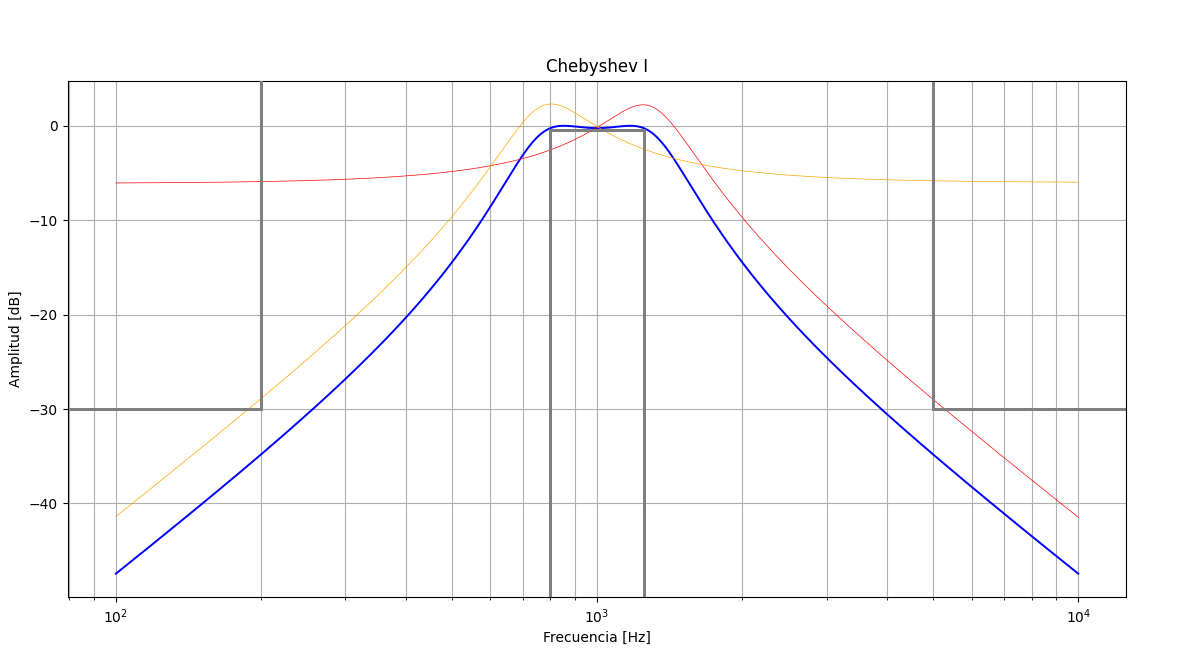
\includegraphics[width=1\linewidth]{figuras/chebyshev_rechazo.png}
    \caption{Diagrama de Bode}
\end{figure}

\hspace{1mm} Se observa la función celeste como el resultado final del circuito implementando ambas funciones (pasa alto y pasa bajo) en simultaneo.

Se cumplen las condiciones de la banda de paso, marcada en verde y las bandas de rechazo marcadas en rojo.\newline

\hspace{1mm} Proceso de creación de los filtros solicitados.

\subsubsection{Filtro Pasabajos}
\begin{verbatim}
	
	      1.642e07
	------------------------
	s^2 + 3184 s + 6.632e07
\end{verbatim}

\begin{figure}[H]
    \centering
    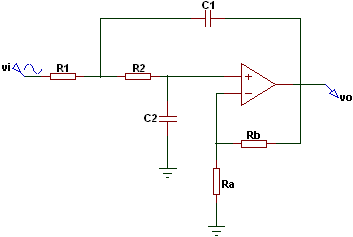
\includegraphics[width=0.75\linewidth]{figuras/pasabajo.teorico.png}
    \caption{Circuito Sallen and Key pasabajos}
    \label{fig:enter-label}
\end{figure}

\hspace{1mm} Utilizando la ley de Kirchhoff de corriente (LCK) realizamos el siguiente sistemas de ecuaciones:
\begin{center}
	$(V_x - V_i) \cdot \frac{1}{R_1} + (V_x - V_o) \cdot sC_1 + (V_x - V^+) \cdot \frac{1}{R_2} = 0$ \\
	$(V^+ - V_x) \cdot \frac{1}{R_2} + (V^+) \cdot sC_2 = 0 $\\
\end{center}
\hspace{1mm} Despejando V+ obtenemos tff y tfb:

\begin{center}
$V^+ = \frac{N}{D} = \frac{V_i \cdot \frac{S}{R1\cdot R_2 \cdot C_1\cdot C_2} + V_o \cdot \frac{S}{R_2 \cdot C_2}}{\frac{1}{R_1 \cdot R_2 \cdot C_1 \cdot C_2} + S \cdot (\frac{1}{R_1 \cdot C_1}+ \frac{1}{R_2 \cdot C_1}+ \frac{1}{R_2 \cdot C_2})+ S^2}$ \\

$T_{ff} = \frac{N_{ff}}{D} = (\frac{V_+}{V_i})_{V0=0} = \frac{\frac{1}{R_1 \cdot R_2 \cdot C_1 \cdot C_2 }}{D}$ \\ 
$T_{fb} = \frac{N_{fb}}{D} = (\frac{V_+}{V_0})_{Vi=0} = \frac{\frac{S}{R_2 \cdot C_2 }}{D}$ \\
\end{center}
\text{Entonces:} \\
\begin{center}
$\frac{V_0}{V_i} = \frac{k \cdot N_{ff}}{D - k \cdot N_{fb}} =  \frac{\frac{k}{R_1 \cdot R_2 \cdot C_1 \cdot C_2}}{S^2+S \cdot \left(\frac{1}{R_1 \cdot C_1} + \frac{1}{R_2 \cdot C_1} + \frac{1}{R_2 \cdot C_2} - \frac{k}{R_2 \cdot C_2}\right) }$

\end{center}
Donde $k = \frac{r_2+r_1}{r_1}$ \\
\hspace{1mm} Igualando los valores a la FT requerida y estableciendo a C un valor típico de 0.1uF obtenemos los valores requeridos de resistores para que se cumpla nuestra función solicitada: \\
 \begin{center}
 $\frac{1}{R_1 \cdot R_2 \cdot C_1 \cdot C_2}$ = 6.632e07 \\
 $\frac{k}{R_1 \cdot R_2 \cdot C_1 \cdot C_2}$ = 1.642e07 \\
 $\frac{1}{R_1 \cdot C_1} + \frac{1}{R_2 \cdot C_1} + \frac{1}{R_2 \cdot C_2} - \frac{k}{R_2 \cdot C_2} = 3184 $ 
\end{center}
\begin{flushleft}
	Establecemos: \\
	$ C_1 = C_2 = 0.1 uF $\\
	$ R_1 = R_2 = R $ \\
\end{flushleft} 

\hspace{1mm}Resolviendo las ecuaciones anteriores podemos obtener:\\
R = 1228 Ohm \\
k = 2.6 \\
\hspace{1mm} Por lo tanto: \\
\begin{center}
 $\frac{k}{R_1 \cdot R_2 \cdot C_1 \cdot C_2}$ = $172.41 \cdot 10^6 \neq 1.642e07$ \\
\end{center}

\hspace{1mm} Debido a que la ganancia obtenida es mayor a la requerida agregamos un atenuador resistivo para que se cumplan todos los requerimientos solicitados.\\
\begin{center}
 Atenuador Resistivo  = 0.095
\end{center}

\[
\alpha = \frac{R_A}{R_A + R_B} = \frac{1.642 \times 10^7}{172.41 \times 10^6} = 0.0952
\]

\hspace{1mm} Debemos mantener \( R_1 = R_A//R_B \)

\[
R_A = \frac{R_1}{\alpha} = 12900 \, \Omega
\]
\[
R_B = \frac{R_1}{1-\alpha} = 1357 \, \Omega
\]

\hspace{1mm} Y para

\[
k = 1 + \frac{R_2}{R_1} = 2.6
\]

\hspace{1mm} \(R_1 = 10 \, \text{k} \Omega \)

\(   R_2 = 16 \, \text{k} \Omega \)

\subsubsection{Filtro Pasa Altos} 

\text{PasaAlto} = \(\frac{s^2}{s^2 + 1896s + 2.35 \times 10^7}\) \\

\begin{figure}[H]
    \centering
    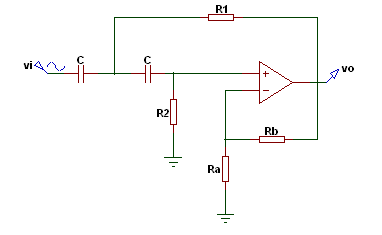
\includegraphics[width=0.75\linewidth]{figuras/filtropasaaltosgen.PNG}
    \caption{Filtro Pasa Alto}
\end{figure}
\hspace{1mm} De igual manera que para el caso del filtro pasa-bajos obtenemos por medio de la ley de kirchhoff de las corrientes las ecuaciones que representan nuestro sistema:

\[
(V_x - V_i)sC_1 + (V_x - V_o)\frac{1}{R_1} + (V_x - V_+)sC_2 = 0
\]

\[
(V_+ - V_x)sC_2 + (V_+)\frac{1}{R_2} = 0
\]

\textbf{Resolviéndolo obtenemos:}

\[
V_+ = \frac{N}{D} = \frac{V_i s^2 + V_o \cdot \frac{s}{R_{IC1}}}{\frac{1}{R_1 R_2 C_1 C_2} + s \left(\frac{1}{R_{IC1}} + \frac{1}{R_{2C1}} + \frac{1}{R_{2C2}}\right) + s^2}
\]

\[
T_{ff} = \frac{N_{ff}}{D} = \left(\frac{V_+}{V_i}\right)_{V_o=0} = \frac{s^2}{D}
\]

\[
T_{fb} = \frac{N_{fb}}{D} = \left(\frac{V_+}{V_o}\right)_{V_i=0} = \frac{\frac{s}{R_{IC1}}}{D}
\]


\hspace{1mm} Entonces:

\[\frac{V_o}{V_i} = \frac{kNff}{D - kNfb} = \frac{k s^2}{s^2 + s \left( \frac{1}{R_1 C_1} + \frac{1}{R_2 C_1} + \frac{1}{R_2 C_2} + \frac{k}{R_1 C_1} \right) + \frac{1}{R_1 R_2 C_1 C_2}}\]


\hspace{1mm} Siendo \( k = \frac{(R_a + R_b)}{R_a} \) 
\bigskip
\newline
 Igualando las ecuaciones obtenidas respecto a los valores solicitados de nuestro sistema y estableciendo a C un valor de 0,1uF obtenemos el los siguientes valores de resistores requeridos para el cumplimiento del filtro pasa altos:

\[
\frac{1}{R_{\text{1}} R_{\text{2}} C_1 C_2} = 2.35 \times 10^7
\]

\[
k \cdot s^2 = s^2
\]

\[
\frac{1}{R_1 C_1} + \frac{1}{R_2 C_1} + \frac{1}{R_2 C_2} - \frac{k}{R_1 C_1} = 1896
\]

\hspace {1mm}Establecemos:

\begin{itemize}
    \item \( C_1 = C_2 = 0.1 \, \mu \text{F} \)
    \item \( k = 1 \)
\end{itemize}

\hspace{1mm}Obtenemos como resultado los siguientes valores de resistores:

\( R_2 = 10548 \, \Omega \)

\( R_1 = 403 \, \Omega \)

\newpage

\section{Simulaciones}

\subsection{Filtro Pasa Bajo}

\begin{figure}[H]
    \centering
    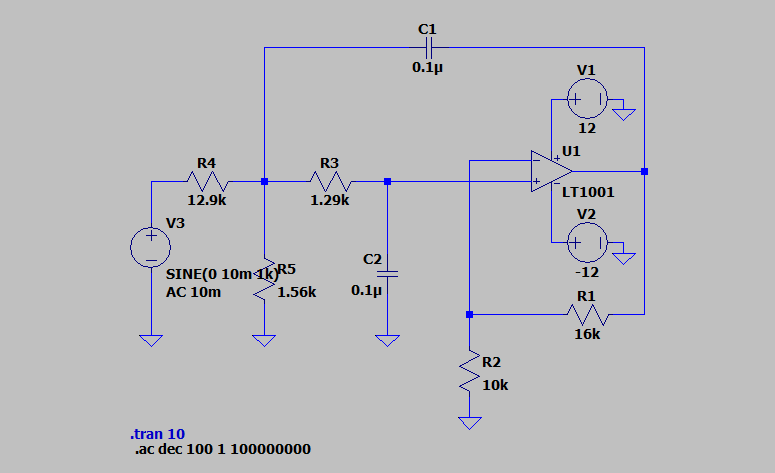
\includegraphics[width=1.0\linewidth]{figuras/pasabajocircuito.png}
    \caption{Circuito filtro Pasa Bajo}
\end{figure}
\begin{figure}[H]
    \centering
    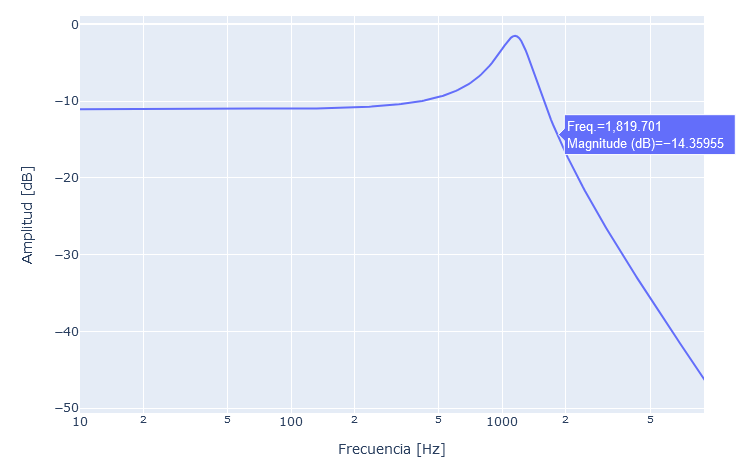
\includegraphics[width=1.0\linewidth]{figuras/diagramas/pasa_bajo_amp.png}
    \caption{Bode filtro Pasa Bajo}
\end{figure}

\begin{figure}[H]
    \centering
    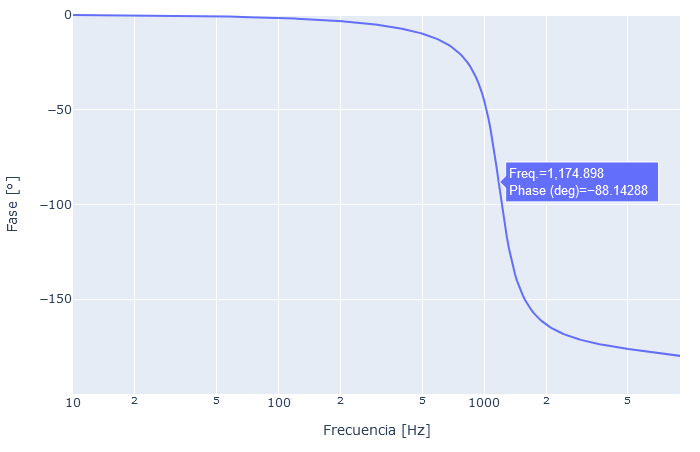
\includegraphics[width=1.0\linewidth]{figuras/diagramas/pasa_bajo_fase.png}
    \caption{Amplitud filtro Pasa Bajo}
\end{figure}

\subsection{Filtro Pasa Alto}

\begin{figure}[H]
    \centering
    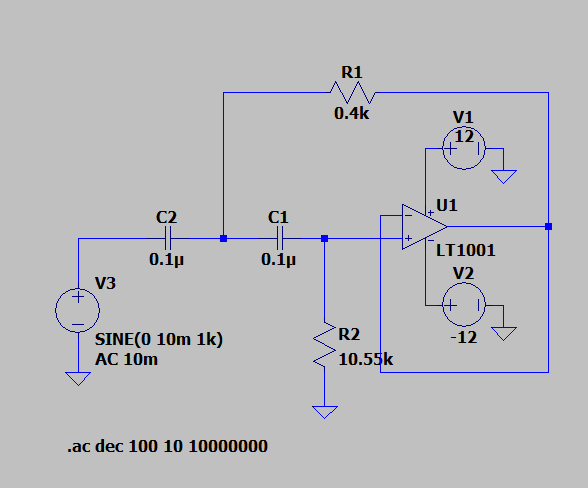
\includegraphics[width=1.0\linewidth]{figuras/pasaaltocircuito.png}
    \caption{Circuito Filtro Pasa Alto}
\end{figure}

\begin{figure}[H]
    \centering
    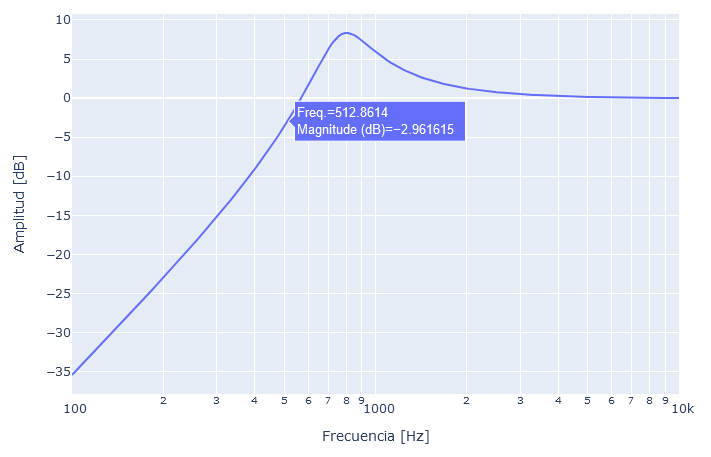
\includegraphics[width=1\linewidth]{figuras/diagramas/pasa_alto_amp.png}
    \caption{Bode Filtro Pasa Alto}
\end{figure}
\begin{figure}[H]
    \centering
    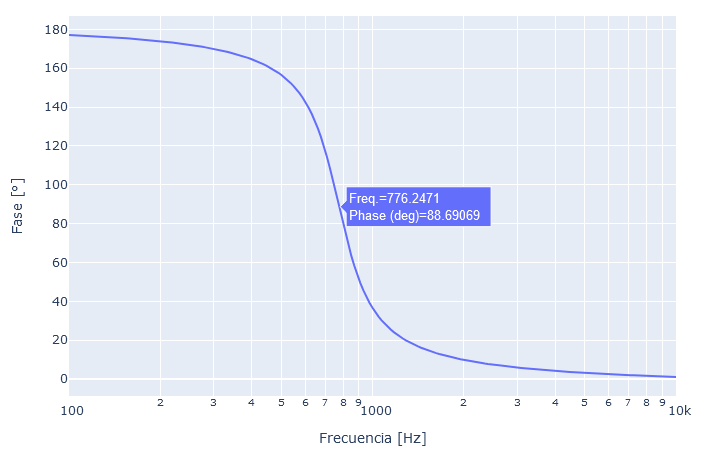
\includegraphics[width=1\linewidth]{figuras/diagramas/pasa_alto_fase.png}
    \caption{Fase Filtro Pasa Alto}
\end{figure}
\newpage

\subsection{Filtro completo Pasa Banda}

\begin{figure}[H]
    \centering
    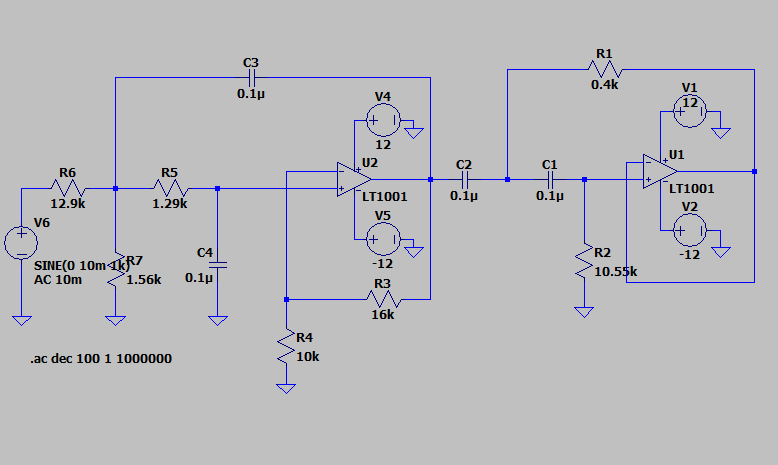
\includegraphics[width=1\linewidth]{figuras/pasabandacircuito.png}
    \caption{Circuito Filtro Pasa Banda}
\end{figure}

\begin{figure}[H]
    \centering
    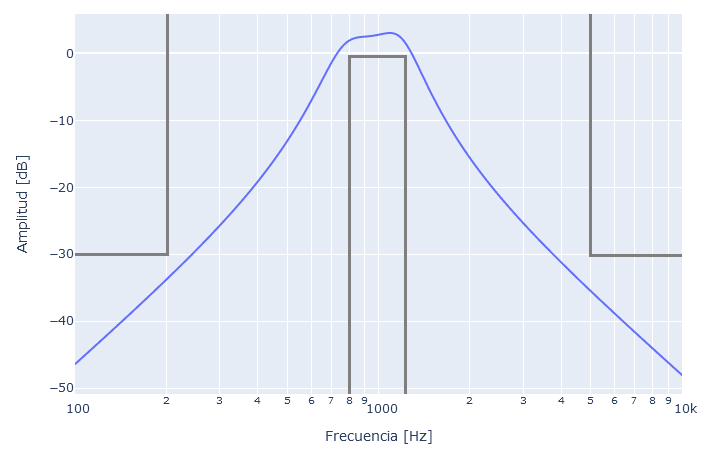
\includegraphics[width=1\linewidth]{figuras/diagramas/pasa_banda_amp.png}
    \caption{Bode Filtro Pasa Banda}
\end{figure}
\begin{figure}[H]
    \centering
    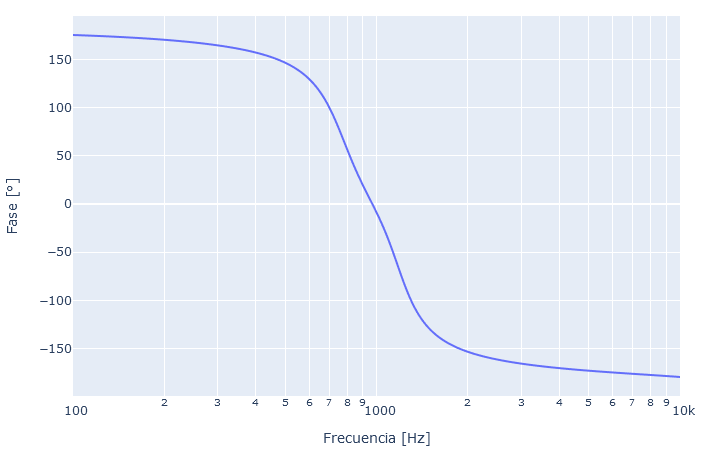
\includegraphics[width=1\linewidth]{figuras/diagramas/pasa_banda_fase.png}
    \caption{Fase Filtro Pasa Banda}
\end{figure}

\hspace{1mm} Pueden observarse las atenuaciones en las frecuencias de nuestro interés: 

\begin{itemize}
\item 800 Hz : -0.240 dB
\item 1250 Hz : -0.466 dB
\item 200 Hz : -34 dB
\item 5000 Hz : -34 dB
\end{itemize}
\hspace{1mm} Las cuales cumplen con los requerimientos del circuito.

\newpage

\section{Cálculo de la sensibilidad}
\hspace{1mm} Para el cálculo de la sensibilidad de la frecuencia del polo (\(\omega_p\)) y el ancho de banda (\(\omega_p / Q_p\)) partimos de la ecuación principal la deducción de \(\omega_p\) la cual es:

\[\omega_p = \sqrt{\frac{1}{R_1 \cdot R_2 \cdot C_1 \cdot C_2}} = \frac{1}{\sqrt{R_1 \cdot R_2 \cdot C_1 \cdot C_2}}\]

\hspace{1mm}Y para el ancho de banda:

\[\frac{\omega_p}{Q_p} = \frac{1}{R_1 C_1} + \frac{1}{R_2 C_1} + \frac{1}{R_2 C_2} - \frac{k}{R_1 C_1}\]

\hspace{1mm}Definimos entonces la sensibilidad según los resistores:

\[
\mathcal{S}\left(\frac{\omega_p}{R}\right) = \frac{\frac{\Delta \omega_p}{\omega_p}}{\frac{\Delta R}{R}} = \frac{R}{\omega_p} \cdot \frac{\partial \omega_p}{\partial R}
\]

\[
\mathcal{S}\left(\frac{\omega_p}{C}\right) = \frac{\frac{\Delta \omega_p}{\omega_p}}{\frac{\Delta C}{C}} = \frac{C}{\omega_p} \cdot \frac{\partial \omega_p}{\partial C}
\]

\[
\mathcal{S}\left(\frac{\frac{\omega_p}{Q_p}}{R}\right) = \frac{\frac{\Delta \omega_p}{\omega_p}}{\frac{\Delta R}{R}} = \frac{R}{\frac{\omega_p}{Q_p}} \cdot \frac{\partial \left(\frac{\omega_p}{Q_p}\right)}{\partial R}
\]

\[
\mathcal{S}\left(\frac{\frac{\omega_p}{Q_p}}{C}\right) = \frac{\frac{\Delta \omega_p}{\omega_p}}{\frac{\Delta C}{C}} = \frac{C}{\frac{\omega_p}{Q_p}} \cdot \frac{\partial \left(\frac{\omega_p}{Q_p}\right)}{\partial C}
\]
 \hspace{1mm} Realizamos una tabla con las sensibilidades correspondientes tomando en cuenta la peor desviación con una tolerancia del 10\% de cada elemento:

\renewcommand{\arraystretch}{1.5}
\begin{table}[H]
\centering
\begin{tabular}{|>{\columncolor[HTML]{B3D9FF}}c|>{\centering\arraybackslash}m{2.5cm}|>{\centering\arraybackslash}m{2.5cm}|>{\centering\arraybackslash}m{3cm}|>{\centering\arraybackslash}m{2.5cm}|}
\hline
\rowcolor[HTML]{B3D9FF} 
     & $\omega_p$ & $\frac{P}{10\%}$ & $\frac{\omega_p}{Q_p}$ & $\frac{P}{10\%}$ \\ \hline
\cellcolor[HTML]{B3D9FF} R1 & $-\frac{1}{2}$ & 5\% & $\frac{-1}{4-K}$ & 18\% \\ \hline
\cellcolor[HTML]{B3D9FF} R2 & $-\frac{1}{2}$ & 5\% & $\frac{-(K-2)}{4-K}$ & 26\% \\ \hline
\cellcolor[HTML]{B3D9FF} C1 & $-\frac{1}{2}$ & 5\% & $\frac{-(K-3)}{4-K}$ & 8\% \\ \hline
\cellcolor[HTML]{B3D9FF} C2 & $-\frac{1}{2}$ & 5\% & $\frac{-1}{4-K}$ & 18\% \\ \hline
\cellcolor[HTML]{B3D9FF} TOTAL & -2 & 20\% & -7 & 70\% \\ \hline
\end{tabular}
\end{table}

\newpage

\section{Análisis de Montecarlo de los componentes}
\hspace{1mm} Para realizar este análisis se varían los valores de los componentes pasivos del circuito de acuerdo a su tolerancia y se toma distribución normal de estos mismo. Se plantea una distribución estadistica del posible valor de la frecuencia del polo de cada etapa ($\omega_p$) , o del ancho de banda correspondiente ($\omega_p$/$Q_p$).

\begin{figure}[H]
    \centering
    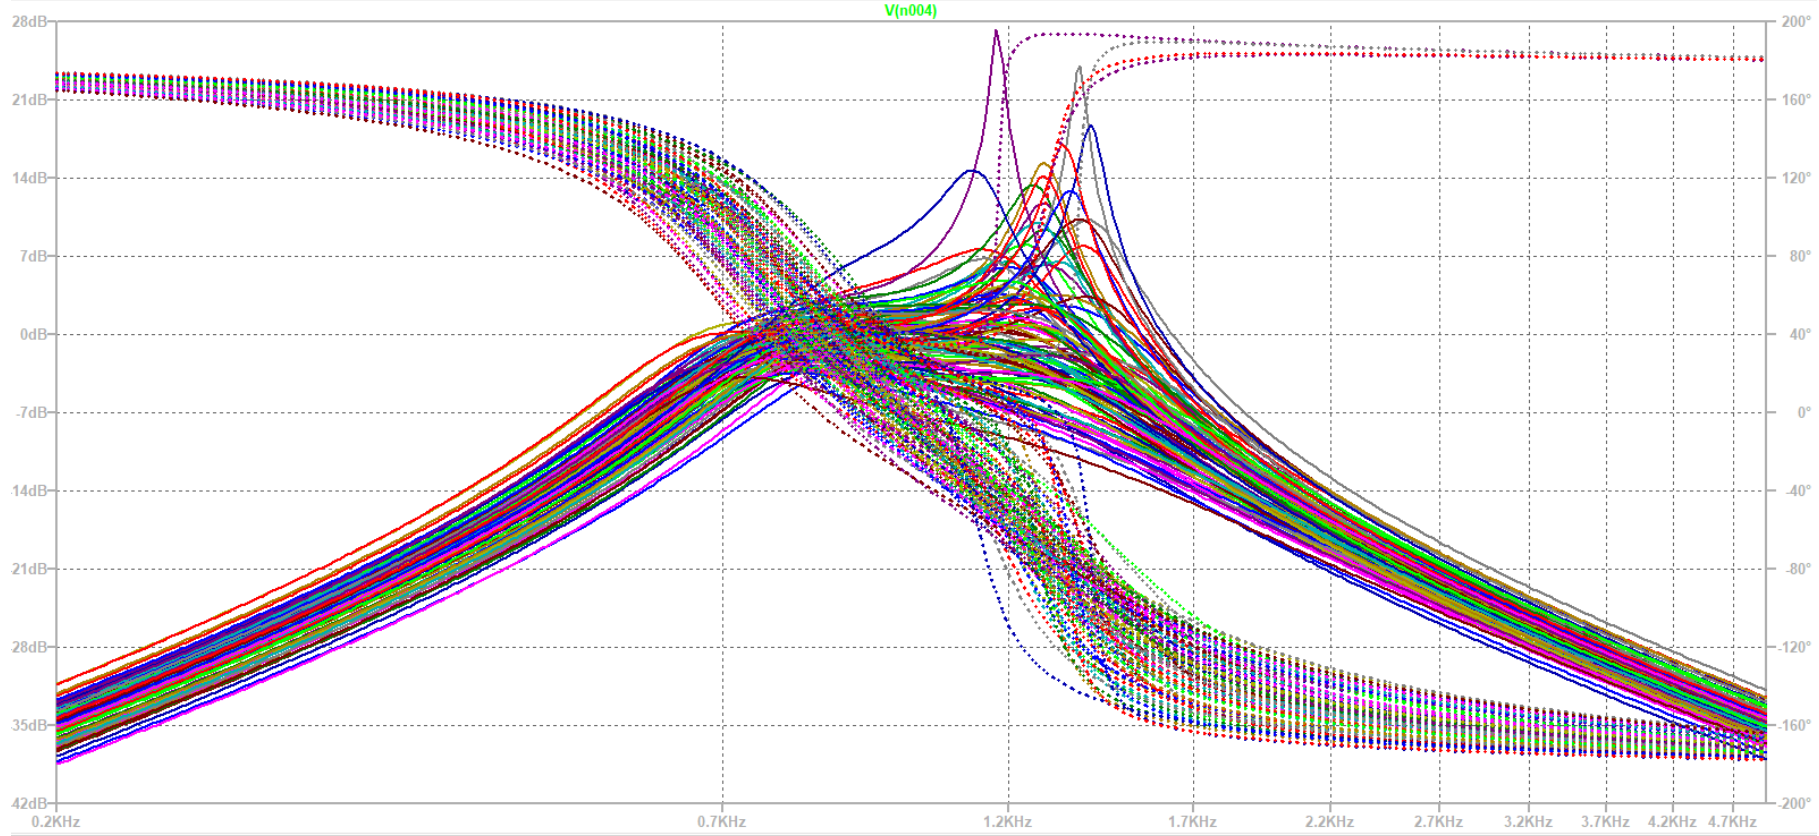
\includegraphics[width=1.0\linewidth]{figuras/AnalisisMontecarlo.PNG}
    \caption{Análisis de Montecarlo}
\end{figure}

\section{Implementación}
El circuito se implemento físicamente en el PCB provisto por el docente. El amplificador operacional seleccionado fue el TL072, montado sobre su respectivo zócalo. El circuito se armó con los componentes con valores normalizados lo más cercano posibles a los valores calculados.

\begin{figure}[H]
    \centering
    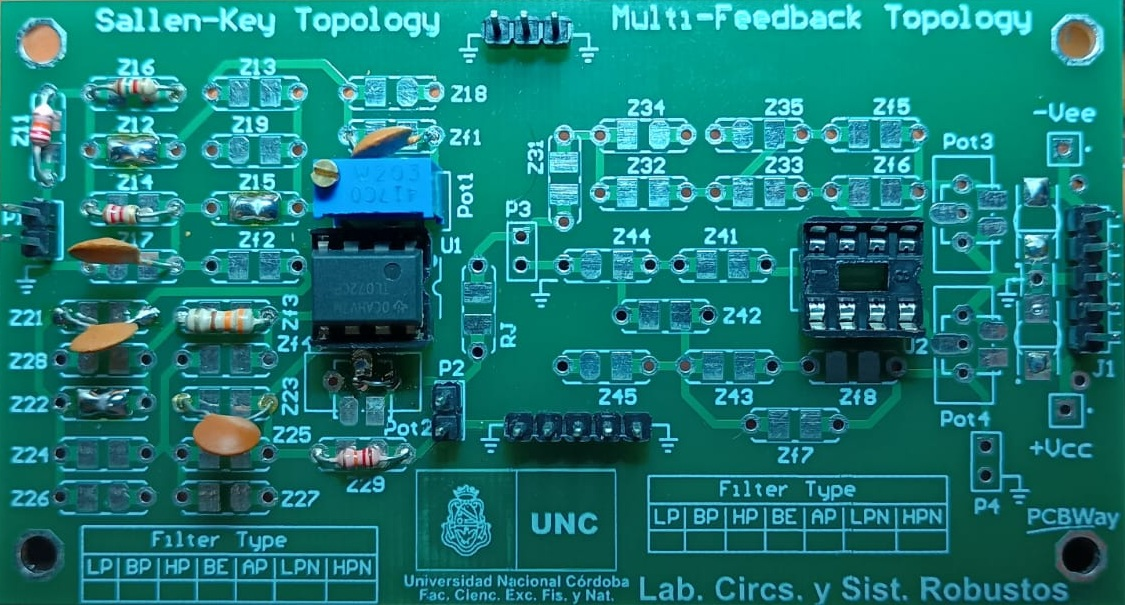
\includegraphics[width=0.75\linewidth]{Filtro pasabanda.jpg}
    \caption{Filtro pasabanda}
    \label{fig:enter-label}
\end{figure}

Se midió la salida del filtro para cuatro frecuencias específicas:
\begin{itemize}
    \item 200 Hz
    \item 800 Hz
    \item 1250 Hz
    \item 5000 Hz
\end{itemize}

Que corresponden a los puntos que describen la banda de paso y la banda de rechazo del filtro. Se ingresó con una señal de 1V de amplitud.

\begin{figure}[H]
    \centering
    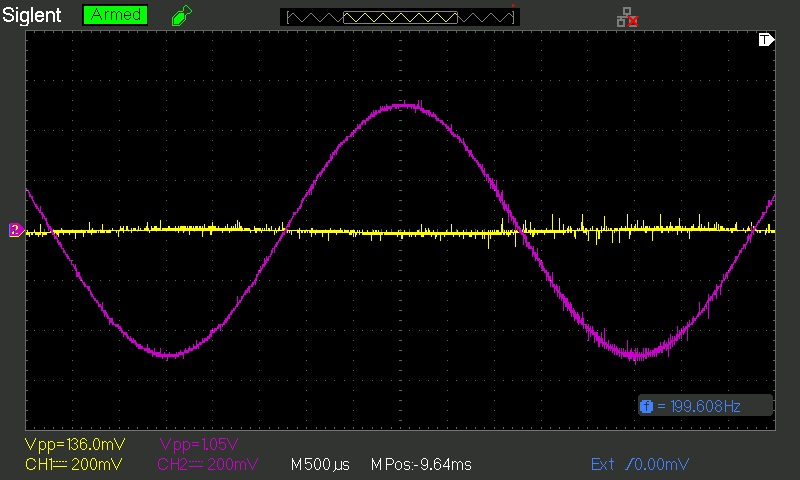
\includegraphics[width=0.75\linewidth]{figuras/SDS00033.jpg}
    \caption{Salida con señal de 200Hz de entrada}
    \label{fig:enter-label}
\end{figure}

La atenuación para esta señal es de 17.75 dB

\begin{figure}[H]
    \centering
    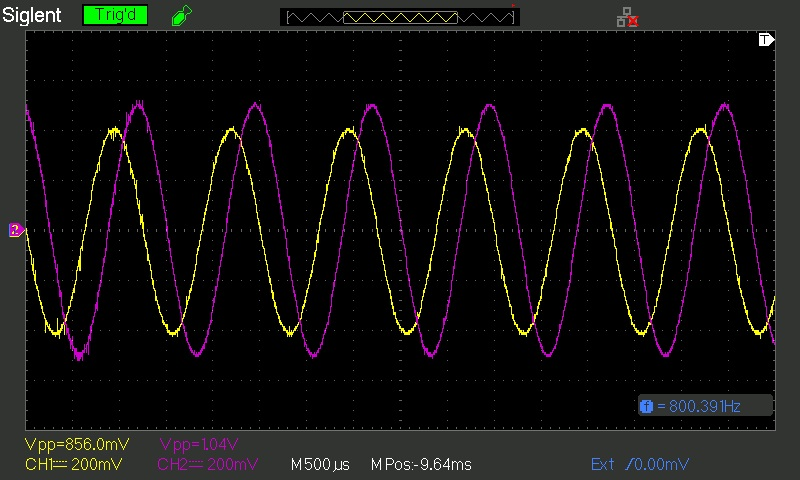
\includegraphics[width=0.75\linewidth]{figuras/SDS00034.jpg}
    \caption{Salida con señal de 800Hz de entrada}
    \label{fig:enter-label}
\end{figure}

En este caso en particular, se observa una atenuación de 1.77 dB

\begin{figure}[H]
    \centering
    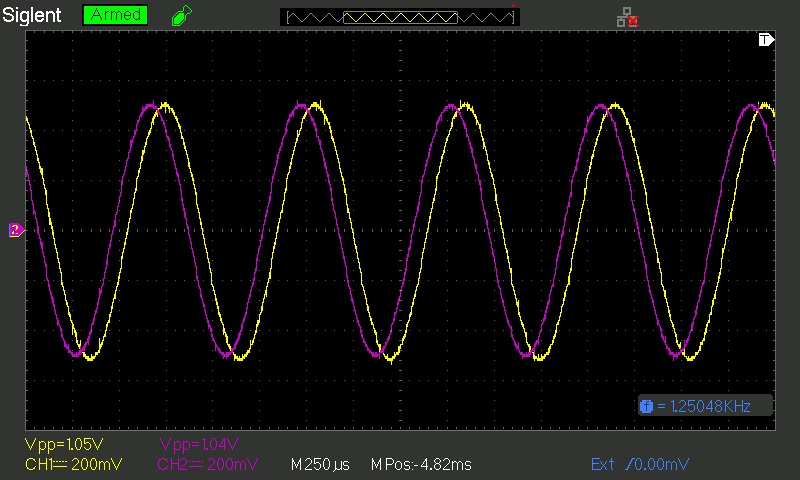
\includegraphics[width=0.75\linewidth]{figuras/SDS00035.jpg}
    \caption{Salida con señal de 1250Hz de entrada}
    \label{fig:enter-label}
\end{figure}

Para esta frecuencia la salida se vio con ganancia unitaria, es decir, el filtro no atenuó la señal (0 dB).

\begin{figure}[H]
    \centering
    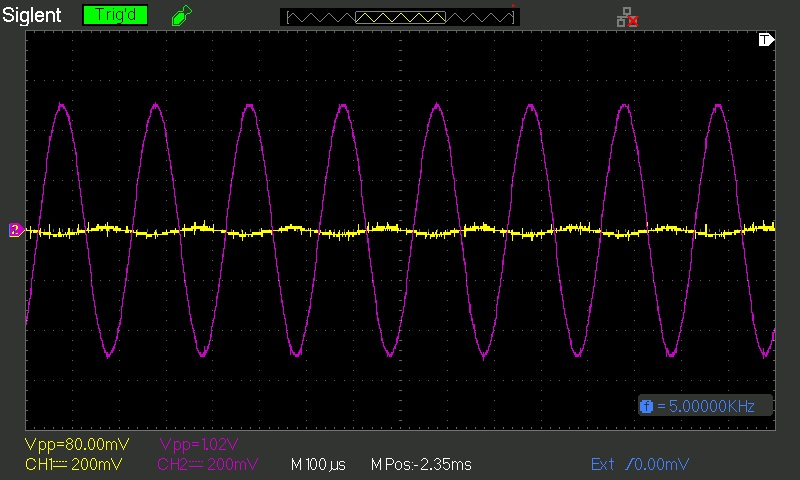
\includegraphics[width=0.75\linewidth]{figuras/SDS00036.jpg}
    \caption{Salida con señal de 5000Hz de entrada}
    \label{fig:enter-label}
\end{figure}

Para el limite inferior de la segunda banda suprimida, se obtuvo una atenuación de 22dB. Finalmente, a modo ilustrativo, se realizó un barrido en frecuencia en la entrada, de 200Hz a 5000Hz para verificar que la señal de salida coincida con la respuesta del filtro.

\begin{figure}[H]
    \centering
    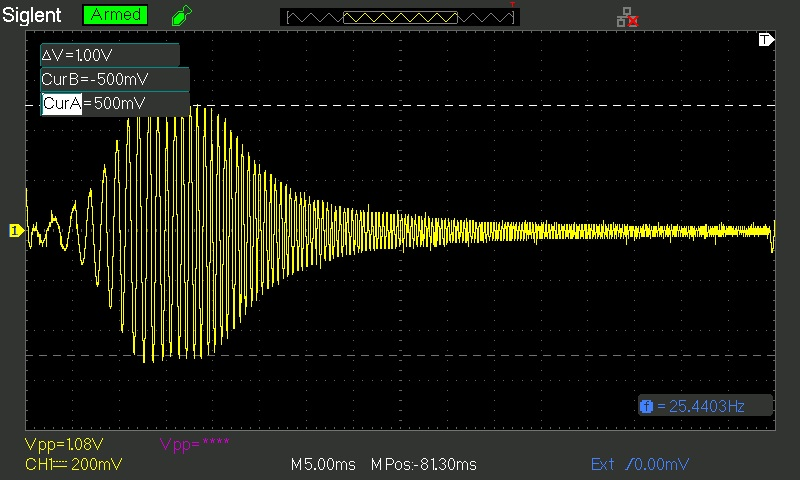
\includegraphics[width=0.75\linewidth]{figuras/SDS00037.jpg}
    \caption{Salida al ingresar un barrido de 200Hz a 5000Hz con un generador de funciones arbitrario}
    \label{fig:enter-label}
\end{figure}


\section{Conclusiones}
\hspace{1mm} El circuito correspondiente al laboratorio numero 4 nos permitió aprender acerca del diseño e implementación de un filtro pasa banda y como las variaciones de los componentes puede llegar a afectar su diseño. Cabe destacar que se realizo el filtro pasa-banda mediante el uso de dos filtros (filtro pasa-bajo y filtro pasa-alto) lo que nos permitió obtener un diseño mas sencillo y a su vez mas eficaz para el sistema solicitado



